% Template for Cogsci submission with R Markdown

% Stuff changed from original Markdown PLOS Template
\documentclass[10pt, letterpaper]{article}

\usepackage{cogsci}
\usepackage{pslatex}
\usepackage{float}

% amsmath package, useful for mathematical formulas
\usepackage{amsmath}

% amssymb package, useful for mathematical symbols
\usepackage{amssymb}

% hyperref package, useful for hyperlinks
\usepackage{hyperref}

% graphicx package, useful for including eps and pdf graphics
% include graphics with the command \includegraphics
\usepackage{graphicx}

% Sweave(-like)
\usepackage{fancyvrb}
\DefineVerbatimEnvironment{Sinput}{Verbatim}{fontshape=sl}
\DefineVerbatimEnvironment{Soutput}{Verbatim}{}
\DefineVerbatimEnvironment{Scode}{Verbatim}{fontshape=sl}
\newenvironment{Schunk}{}{}
\DefineVerbatimEnvironment{Code}{Verbatim}{}
\DefineVerbatimEnvironment{CodeInput}{Verbatim}{fontshape=sl}
\DefineVerbatimEnvironment{CodeOutput}{Verbatim}{}
\newenvironment{CodeChunk}{}{}

% cite package, to clean up citations in the main text. Do not remove.
\usepackage{cite}

\usepackage{color}

% Use doublespacing - comment out for single spacing
%\usepackage{setspace}
%\doublespacing


% % Text layout
% \topmargin 0.0cm
% \oddsidemargin 0.5cm
% \evensidemargin 0.5cm
% \textwidth 16cm
% \textheight 21cm

\title{Reaction times as a measure of developmental pragmatic implicature
processing}


\author{{\large \bf Rose M. Schneider} \\ \texttt{rschneid@stanford.edu} \\ Department of Psychology \\ Stanford University \And {\large \bf Michael C. Frank} \\ \texttt{mcfrank@stanford.edu} \\ Department of Psychology \\ Stanford University}

\begin{document}

\maketitle

\begin{abstract}
Children's difficulty with scalar implicatures -- inferences from a
weaker lexicalized description that a stronger alternative is true --
are a puzzle in pragmatic development. Previous research indicates that
children's failures in processing scalar implicatures may be rooted in
an unestablished quantifier scale, with children who struggle with the
quantifier ``some'' being unable to contrast different quantifiers to
make the implicature. However, the source of this failure is unclear.
Here, we explore reaction time as a measure of processing for scalar
implicatures (and reasoning about salient alternatives, such as
``none''). In our analyses, we explore overall performance and reaction
time patterns across development, finding that increased reaction times
and accuracy for the quantifiers ``some'' and ``none.'' Motivated by
these findings, we use a Drift Diffusion Model to explore the
relationship between accuracy and reaction time in processing both
scalar implicatures, and the quantifiers ``some'' and ``none'' more
broadly. Overall, we find evidence that while children's performance in
scalar implicature tasks is hindered by absent quantifier knowledge,
their success also requires additional processing when reasoning about
that quantifier scale.

\textbf{Keywords:}
Pragmatics; development; language.
\end{abstract}

\section{Introduction}\label{introduction}

To successfully comprehend speech, listeners frequently make inferences
which go beyond the literal meaning of a speaker's utterance. In the
case of \emph{pragmatic implicatures} (Grice, 1975), a weaker literal
description can imply that a stronger alternative is true. Thus, an
adult listener would strongly infer from the statement ``I enjoyed
\emph{some} of my winter break'' that some (but not \emph{all}) of my
break was pleasant. This \emph{scalar implicature} (SI) relies heavily
on a knowledge of the relevant lexical alternatives in the quantifier
scale \(<\)none, some, all\(>\), as a listener must be able to contrast
these alternatives in computing the implicature. While scalar
implicatures are easily comprehended by adults, they pose a pragmatic
challenge to children until fairly late in development. What is the
source of children's difficulties with scalar implicatures?

In contrast to adults' spontaneous processing of such pragmatic
implicatures, children display marked and striking failures in such
tasks. For example, when judging a scene in which three of three horses
have jumped over a fence, preschoolers are likely to endorse the
statement ``\emph{All} of the horses jumped over the fence'' as
felicitous, rather than the appropriate statement ``\emph{Some} of the
horses jumped over the fence'' (Papafragou \& Musolino, 2003). Across
different studies, however, children exhibit varying performance,
depending on the paradigm, syntactic construction of the implicature
prompts, access to visual and lexical alternatives, and age (Guasti et
al., 2005; Horowitz \& Frank, 2015; Noveck, 2001; Papafragou \&
Musolino, 2003; Papafragou \& Tantalou, 2004). Making inferences from
these various datasets about the source of children's failures in making
scalar implicatures is made difficult by various measures and tasks
uses.

In an attempt to reconcile these various accounts, Horowitz and Frank
(2015) designed a simple referent selection paradigm that could be used
across a broad age range (3--5 years) to explore lexicalized (scalar)
implicatures. In this task, children saw three book covers, each
featuring four familiar objects (Figure \ref{fig:image}), and the
experimenter described a book using either a scalar (quantifier)
description (e.g., ``On the cover of my book, \emph{none/some/all} of
the pictures are cats.''). Children's responses were scored as correct
if they selected the book consistent with the quantifier description.

\begin{CodeChunk}
\begin{figure}[H]

{\centering 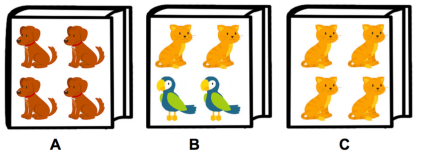
\includegraphics{figs/image-1} 

}

\caption[Example trial stimuli used in Horowitz and Frank (2015)]{Example trial stimuli used in Horowitz and Frank (2015).}\label{fig:image}
\end{figure}
\end{CodeChunk}

Using this paradigm, Horowitz and Frank found children struggled with
the quantifiers ``some'' and ``none'' in relation to ``all'', although
performance increased across development. Intriguingly, they found that
performance between these two quantifiers was strongly bimodal and
correlated: Children who failed on trials with the quantifier ``some''
similarly struggled with ``none,'' and vice versa.

Children's failures in computing scalar implicatures, and their related
performance processing the quantifiers ``some'' and ``none'' presented
two hypotheses for sources of developmental difficulty in this task,
namely, lack of quantifier knowledge and developing inhibitory control
(Horowitz, Schneider, \& Frank, In prep.). Horowitz et al. explored
these two hypotheses in an individual differences task, running their SI
(Horowitz \& Frank, 2015) task in conjunction with quantifier-knowledge
(Barner, Chow, \& Yang, 2009) and inhibitory control (Zelazo, 2006)
tasks. Overall, they found that children's struggles in the SI task was
strongly correlated with quantifier knowledge, even when controlled for
age. While inhibitory control was strongly correlated with age, it was
not related to children's performance on the SI task (Horowitz et al.,
In prep.).

While the ability to compute a scalar implicature seems to be closely
related to knowledge of the complete quantifier scale (rather than oure
inhibitory control), it is likely that children's failures have several
underlying causes. In particular, an unexplored (and more nuanced)
measure of inhibitory control is the response latency associated with a
given quantifier.

Here, we explore children's response times in Horowitz and Frank's
(2015) task as a measure of inhibitory control. To obtain accurate
reaction times, we adapted the task for an iPad, and expanded the sample
size. In our analyses, we explore overall accuracy and patterns of
performance, as in (Horowitz \& Frank, 2015; Horowitz et al., In prep.).
Additionally, we examine reaction time patterns across all quantifier
types, and whether correctly processing quantifiers correctly entails a
longer response latency (and additional processing). Finally, we use a
Drift Diffusion Model to explore accuracy and reaction times on a scalar
implicature task across development.

\section{General Methods}\label{general-methods}

In this study, we adapted a Scalar Implicature paradigm developed by
Horowitz and Frank (2015) for the iPad. In addition to capturing
detailed reaction time data, this version included more trials, and
standardized prosody across all trials, in addition to a completely
randomized design.

\subsubsection{Participants}\label{participants}

94 out of a planned sample of 120 was recruited from Bing Nursery School
at Stanford University and the Children's Discovery Museum in San Jose.
Participants ranged in age from 3--6.5 years: 11 3--3.5-year-olds (M =
3.28, median = 3.27, SD = 0.16); 19 3.5--4-year-olds (M = 3.8, median =
3.79, SD = 0.14); 20 4--4.5-year-olds (M = 4.28, median = 4.29, SD =
0.16); 25 4.5--5-year-olds (M = 4.75, median = 4.74, SD = 0.16); and 19
5--6.5-year-olds (M = 5.64, median = 5.63, SD = 0.37). Two additional
children were run, but were excluded as out of the age range. Based on
(Horowitz \& Frank, 2015; Horowitz et al., In prep.), the initially
planned sample size was 96 children from 3--5 years. After collecting
data from 57 participants, however, we observed significantly lower
performance on critical trials across all age groups, indicating that
the iPad adaptation of the scalar implicature task was slightly more
challenging for all children. With this extended developmental
trajectory in mind, we decided to include an older age group of
twenty-four 5--6.5-year-olds.

\subsubsection{Stimuli}\label{stimuli}

General format of the task was identical to (Horowitz \& Frank, 2015),
with the exception of added items for additional trials. The study was
programmed in HTML, CSS, and JavaScript, and displayed to children on
full-sized iPad. Each trial displayed three book covers, each containing
a set of four familiar objects (Figure \ref{fig:image}). Each trial
allowed 2.5s for children to visually inspect the three book covers,
before the experiment played the trial prompt (e.g., ``On the cover of
my book, \emph{none} of the pictures are cats.''). Each trial was
completely randomized, with the exception that similar items were
displayed together (e.g., food, clothing). Each session involved 30
trials, with 10 trials per quantifier-type (``all'', ``some'', and
``none''). In our randomization, quantifier triad order, items (within
category), target item, and quantifier, were randomized for all
participants.

\subsubsection{Procedure}\label{procedure}

Sessions took place individually in a small testing room away from
either the museum or the nursery school. Each session began with the
child playing the ``dot game,'' which required them to press dots on the
iPad screen as fast as they could. This game was included to familiarize
children with the iPad. After children finished the dot game, the
experimenter introduced them to ``Hannah,'' who wanted to play a
guessing game with her books. The experimenter explained that Hannah
would show the child three books, and would give the child \emph{one}
hint about which book she was thinking of. The experimenter emphasized
that Hannah would only give one hint, so they had to listen carefully.
Children then saw a practice trial with three books featuring a
refrigerator, a TV, and a couch. After 2.5s, a female voice said ``On
the cover of my book there's a TV.'' Once children correctly made their
selection, a green box appeared around the selection. Children moved
trials along at their own pace by pressing a green button that appeared
after they had made their selection.

Reaction times were measured from the onset of the target word. Each
audio clip used the same three frames (e.g., ``On the cover of my book,
\emph{some} of the pictures\ldots{}'') so that prodosdy was emphasized
equally across all trials. Across all trials, the average length of each
audio clip (including target item phrase, e.g., ``\ldots{}are cats'')
was approximately 6s. In all, there were 270 different target items.
Children could only make one selection. If a child was not paying
attention, or if she did not hear Hannah's prompt, the experimenter
repeated it, matching the original prosody.

\section{Results}\label{results}

In analyzing the results, we excluded any trials in which reaction time
exceeded thirty seconds, which indicated that the child had missed the
prompt, or was not paying attention. After this initial cut, we excluded
responses outside three standard deviations of the log of the reaction
time mean. This cleaning process resulted in a data loss of XX trials
(XX\%).

\subsection{Accuracy}\label{accuracy}

\begin{CodeChunk}
\begin{figure}[h]
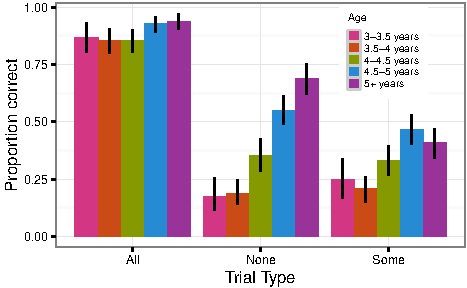
\includegraphics{figs/overll_acc-1} \caption[Children's overall accuracy for each quantifier type]{Children's overall accuracy for each quantifier type. Bars show mean performance for each age group. Error bars are 95 percent confidence intervals computed by non-parametric bootstrap.}\label{fig:overll_acc}
\end{figure}
\end{CodeChunk}

In our first planned analysis, we explored children's overall patterns
of accuracy for each quantifier type. Figure \ref{fig:overall_acc} shows
children's performance for each quantifier type. For each age group, we
see significantly lower accuracy for the quantifiers ``some'' and
``none'' (t-test stats will go here when sample is complete). In a
comparison with previous results using this paradigm (Horowitz \& Frank,
2015; Horowitz et al., In prep.), we found lower performance for
``some'' and ``none'' trials, indicating that the iPad adaptation of the
paradigm was slightly more difficult for preschoolers.

\subsubsection{Statistical modeling}\label{statistical-modeling}

(Logistic regression model will go here - overall, children do better
with age, but worse on some and none trials; however, they do better on
these trials as they get older. Data still coming in, and model is not
converging yet because it's a bit sparse).

\subsubsection{Correlation between ``some'' and
``none''}\label{correlation-between-some-and-none}

(Correlation info goes here - again, sparse data in youngest and oldest
age bins, but observing a positive correlation between ``some'' and
``none'' trials, as we did in previous version of this study. Also
address bimodal performance on these trials when data is clearer.)

\subsection{Reaction time analyses}\label{reaction-time-analyses}

Children's reaction times on this task may be a measure of the
processing a particular quantifier entails. We measured reaction times
in milliseconds on each trial, following the onset of the target noun.

\subsubsection{Developmental reaction time
distribution\\}\label{developmental-reaction-time-distribution}

Figure \ref{fig:rt_spread} shows the distribution of reaction times for
each quantifier, faceted by age group. Overall, we found that reaction
times decreased with age (fill in with more data about developmental
differences).

Figure \ref{fig:density} shows the density of reaction times for correct
and incorrect selections for each quantifier type. We find a higher
distribution of fast reaction times across all age groups for ``all''
trials, and evidence of a speed-accuracy tradeoff in older age groups
for ``some'' and ``none'' trials. (More information about these, and
motivation for diffusion after more data is collected).

(Address correlation between reaction times and responses on certain
trial types as a segue into statistical models).

\subsubsection{Statistical models}\label{statistical-models}

We ran a mixed effects model (final formula goes here) predicting
response time as an interaction of age, trial number, and trial type.
(Final numbers go here; we find that with current dataset, children are
faster with age, but slower with None and Some trial types.
Interestingly, we find that that children are still slower with age on
none and some trials; this is particularly interesting because in our
previous accuracy model, we found increased performance on these trial
types. This indicates that older children are taking longer to respond
to these trial types, but are more likely to get them correct. This is
an important motivation in the diffusion modeling, because it is unclear
as to what is driving this pattern of performance.)

\subsection{Drift diffusion models}\label{drift-diffusion-models}

In our previous statistical models, we observed a speed-accuracy
tradeoff in older children's performance on ``some'' and ``none''
trials. This suggests that children may be taking more time to process
these particular quantifiers as they become more familiar with the
quantifier scale. A drift diffusion model (DDM) can provide a more
detailed view of the relationship between accuracy and reaction time in
behavioral tasks (Milosavljevic, Malmaud, Huth, Koch, \& Rangel, 2010).
In the following DDM, we explore reaction time as an indication of the
processing time involved with the quantifiers in this task. (Diffusion
models aren't done, so they will go here).

\section{General Discussion}\label{general-discussion}

We adapted a previously validated scalar implicature task (Horowitz \&
Frank, 2015; Horowitz et al., In prep.) for the iPad to explore whether
children's success in this task was a result of increased processing
time with the quantifiers ``some'' and ``none.'' In our analyses, we
found that children were overall less accurate when evaluting the
quantifiers ``some'' and ``none,'' but that their performance increased
with age. Interestingly, in our reaction time analyses, we found an
interaction between reaction time and age, with older children taking a
slightly longer time to respond to these trials, but ultimately being
more accurate. (DDM summary here).

Our work contributes to the existing literature in utilizing a novel
method to collect accurate and detailed reaction time data on a scalar
implicature task. Response latencies are an important indicator of the
pragmatic challenges that children face in processing implicatures.
Additionally, our findings replicate previous work, providing evidence
for the appropriateness of this paradigm in targeting scalar
implicatures. Further, our larger sample size, increased number of
trials, and randomized design strengthen our analytical power, and allow
for more detailed inferences from the data.

(More detailed conclusions will go here, once all analyses are
complete).

\section{Acknowledgements}\label{acknowledgements}

Special thanks to Bing Nursery School, the San Jose Children's Discovery
Museum, Veronica Cristiano, Rachel Walker, and Tamara Mekler for their
help with data collection.

\section{References}\label{references}

\setlength{\parindent}{-0.1in} \setlength{\leftskip}{0.125in} \noindent

Barner, D., Chow, K., \& Yang, S. (2009). Finding one's meaning: A test
of the relation between quantifiers and integers in language
development. \emph{Cognitive Psychology}, \emph{58}(2), 195--219.

Grice, H. (1975). \emph{Logic and conversation} (pp. 41--58).

Guasti, M., Chierchia, G., Crain, S., Foppolo, F., Gualmini, A., \&
Meroni, L. (2005). Why children and adults sometimes (but not always)
compute implicatures. \emph{Language and Cognitive Processes},
\emph{20}(5), 667--696.

Horowitz, A., \& Frank, M. C. (2015). Sources of developmental change in
pragmatic inferences about scalar terms. In \emph{Proceedings of the
37th annual conference of the cognitive science society.}

Horowitz, A., Schneider, R. M., \& Frank, M. C. (In prep.). The trouble
with quantifiers: Children's difficulties with ``some'' and ``none''.

Milosavljevic, M., Malmaud, J., Huth, A., Koch, A., \& Rangel, A.
(2010). Drift diffusion model can account for accuracy and reaction time
of value-based choices under high and low time pressure. \emph{Judgment
and Decision Making}, \emph{5}(6), 437--449.

Noveck, I. (2001). When children are more logical than adults:
Experimental investigations of scalar implicature. \emph{Cognition},
\emph{78}(2), 165--188.

Papafragou, A., \& Musolino, J. (2003). Scalar implicatures: Experiments
at the semantics-pragmatics interface. \emph{Cognition}, \emph{86}(3),
253--282.

Papafragou, A., \& Tantalou, N. (2004). Children's computation of
implicatures. \emph{Language Acquisition}, \emph{12}, 71--82.

Zelazo, P. D. (2006). The dimensional change card sort (dCCS): A method
of assessing executive function in children. \emph{Nature Protocols},
\emph{1}, 297--301.

\end{document}
